% ##################################################################################################################
\chapter{Samara}
\label{ch:samara}
\hfill \textbf{Authors:} Oleg Saprykin, Olga Saprykina, Tatyana Mikheeva

% ##################################################################################################################
\section{Study Area}
Samara is a major Russian city, regional capital of the Samara region, situated on the left bank of the Volga River between the mouths of the Samara and Sok rivers. The area is 466\,square kilometers, made up of nine administrative districts, with a city population of  1\,172\,348\,people (year~2014). There are more than 2.7\,million people living within the city agglomeration \citep[][]{GKS_2010}.

Personal and public transportation are developed to varying degrees in Samara city. Auto-mobilization of the population is 286\,vehicles per 1\,000\,people (year~2014) \citep[][]{Gradoteka_2015}. Public transport consists of trams, buses, trolleybuses and subway. Transit of freight through the city is prohibited.

Samara is a major economic, transport, scientific, educational and cultural center. However, despite this, the city's street and road network is insufficiently developed, leading to the following problems.

\begin{itemize}
\item The street and road network has only two highways, which are connected by narrow streets; there are no transverse highways, resulting in traffic congestion. According to research from the Yandex company, Samara city was in fourth place for number of traffic jams in Russian cities \citep[][]{Yandex_2013}.
\item Lack of sufficient parking areas leads to parking along city roads, creating additional traffic congestion.
\item Active construction development in~2000, characterized by absence of an overall city building strategy, led to obvious violations in transport planning and significantly degraded  transport infrastructure quality.
\item Samara is located opposite the Samarskay Luka National Park, a region of unique natural beauty, but a destination for a huge number of summer weekend recreational trips, leading to uneven traffic flow distribution in the region.
\end{itemize}

In addition to these problems, Samara city is currently attempting to move toward more sustainable development, which raises new challenges:
\begin{itemize}
\item rapid growth of residential development within the city boundaries requires transport infrastructure modification,
\item formation of new neighborhoods and new cottage villages within the urban agglomeration involves the construction of new roads, bridges and interchanges,
\item hosting the FIFA-2018 World Cup requires traffic management organization in the downtown, stadium and festival/fans areas.
\end{itemize}

These issues and developments require street and road network modernization, impossible without traffic flow simulation modeling to support the projects.

% ##################################################################################################################
\section{Transport Demand}
Population residence coordinates were taken from anonymized city population spatial distribution information provided by the National Population Census~2010 \citep[][]{GKS_2010}. Place of employment coordinates about Samara region companies and organizations were based on data from address directories.

Statistic package R was used for \gls{od} matrices calculation; initial data relied on collected information about population distribution and employment locations. The estimation of \gls{od} matrices was performed by the entropy model using the Shelehovsky-Shtskiy balance method \citep[][]{Nurminski_2009, Autodor_2013, Shvetsov_2003}. This approach is applicable for estimation of the \gls{od} matrices values in case worker, business or recreation trips for private vehicles or freight transport. The \gls{od} matrix was then obtained, which showed number of agents moving from one transport zone to another.

Activity chains were calculated for define path of each \gls{matsim} agent. Activity chains calculation was performed by a custom-developed method, using the author's algorithm described in \citet[][]{SaprykinaEtAl_2012}. Activity chains calculation uses \gls{od} matrices as source data and resulting data was kept in the plans file and used in \gls{matsim}.

% ##################################################################################################################
\section{Transport Supply}
As shown in Figure~\ref{fig:samara_fig1}, the road network was extracted from \gls{osm} and saved to the \gls{matsim} network format, using the \lstinline|NetworkEditor| module presented in Chapter~\ref{ch:contrib-networkEditor}. 
%\ah{Ref. which one?} \ah{according to Oleg's mail it was the ``old'' editor} 
Detailed verification of the obtained network model revealed that some roads have incorrect number of lanes, requiring the writing of a utility that semi-automatically allowed for adjustment of the street and road network model according to the actual transportation planning scheme. Minor model inaccuracies were corrected manually in the \lstinline|NetworkEditor|. The final network model consists of 4\,365\,nodes and 11\,178\,links.
%
 %------------
\createfigure%
{The transport network extraction process}%
{The transport network extraction process}%
{\label{fig:samara_fig1}}%
{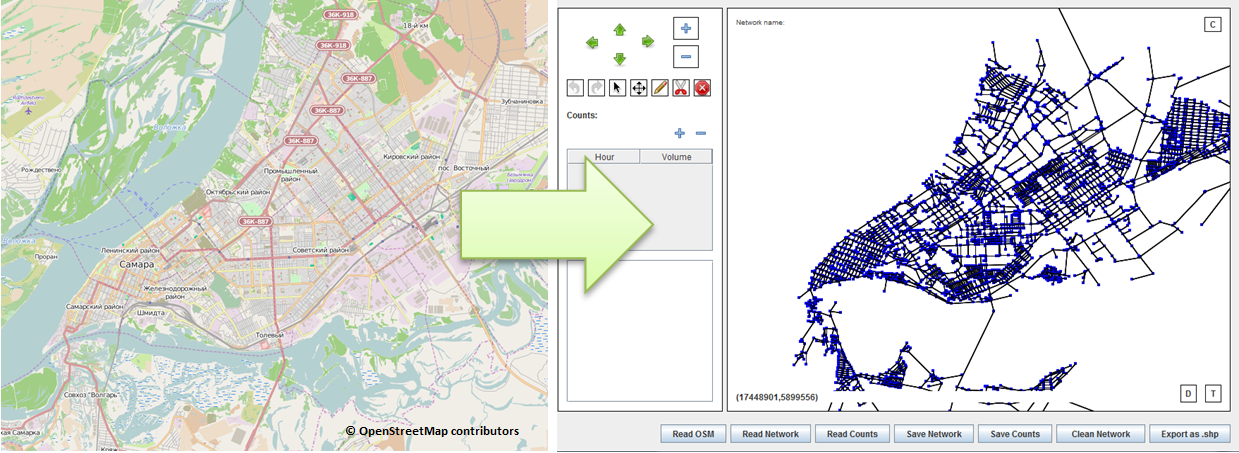
\includegraphics[width=0.99\textwidth, angle=0]{./scenarios/figures/samara_fig1.png}}%
{}
 %------------

The network model should contain transport infrastructure elements for adequate transportation planning reflection. The model takes into account certain traffic signs: speed limit, traffic lanes, movement on the interceptions and ``no entry''. Addition of traffic lights to the model is under development now. At this point, traffic light regulation schemes at specific intersections have been developed; work on their integration into the general city model is underway.

Transport simulation was performed only for private vehicles; Inclusion of public transport to the model is in process. Bicycle paths are still poorly developed in the city; therefore, their simulation is ow-priority. 

% ##################################################################################################################
\section{Calibration and Validation}
For calibration purposes, information about traffic flows at all intersections of Krasnoglinskoye highway and Voljskoe highway, as well as the intersections of central (historical) part of the city, was used. Traffic flow intensity data was received for the period from 19th to 24th of May~2009. Source data required pre-processing, which consisted of vehicle number alignment  according to their type and calculation of total intensity in the target area. Maximum intensity requirement was utilized because intensity measurements were performed during ``rush hours'' from 8\,am to 11\,am and from 4\,pm to 7\,pm \citep[][]{Mikheeva_2008}. 

For transport infrastructure mode validation and verification of its accuracy vs. real traffic conditions in the city, the following steps were completed: 
\begin{itemize}
\item traffic flow parameters field measurements,
\item data gathered from different traffic Web-services (Yandex Maps, Google Maps, etc.),
\item comparative analysis of results obtained from the simulation, field explorations and Web-services \citep[][]{SaprykinaEtAl_2014}.
\end{itemize}

% ##################################################################################################################
\section{Intelligent Traffic Analysis}
 The simulation results analysis is especially valuable to solve the relevant problems. 
With \gls{matsim}'s tools Senozon \gls{via} (Chapter~\ref{ch:via}) and \gls{otfvis} (Chapter~\ref{ch:otfvis}), visual analysis of the model can be performed. 
However, a deeper understanding of the model can be achieved by applying data mining tools to simulation results to 
identify hidden patterns and correlations, supplying more information to address applied problems. 

At this point, the simulation output folder contains files with events and actual plans, containing all actions performed by agents. For loading the data to the mathematical package R, they were converted into \lstinline|.csv| format through specially designed utility and MS Excel applications. Transport infrastructure information from external sources was also imported to~R as a table, containing the coordinates and types of the object. This made it possible to process the \gls{matsim} output using all power of the programming language~R.

The search for hidden patterns was performed using the \lstinline|NeuralNet| package installed in R. One of the goals was finding dependencies of tension at transport flows' gravity points from transport infrastructure spatio-temporal parameters. To solve this problem, a feed-forward neural network was used, trained by resilient back-propagation with weight backtracking algorithm. Source data was split into training and test sets in a 70/30 ratio. Verification was carried out by the regularity criterion \citep[][]{MikheevaEtAl_2012}.

The study produced a trained neural network, able to predict gravity points' tension during changing transport infrastructure parameters. This eliminates the need to restart the simulation to test the hypotheses for city transport infrastructure changes, allowing an overview of changes on the fly. Figure~\ref{fig:samara_fig2} shows how the trained neural network displays the tension calculation process at the intersection.

 %------------
\createfigure%
{The tension calculation process by the trained neural network}%
{The tension calculation process by the trained neural network}%
{\label{fig:samara_fig2}}%
{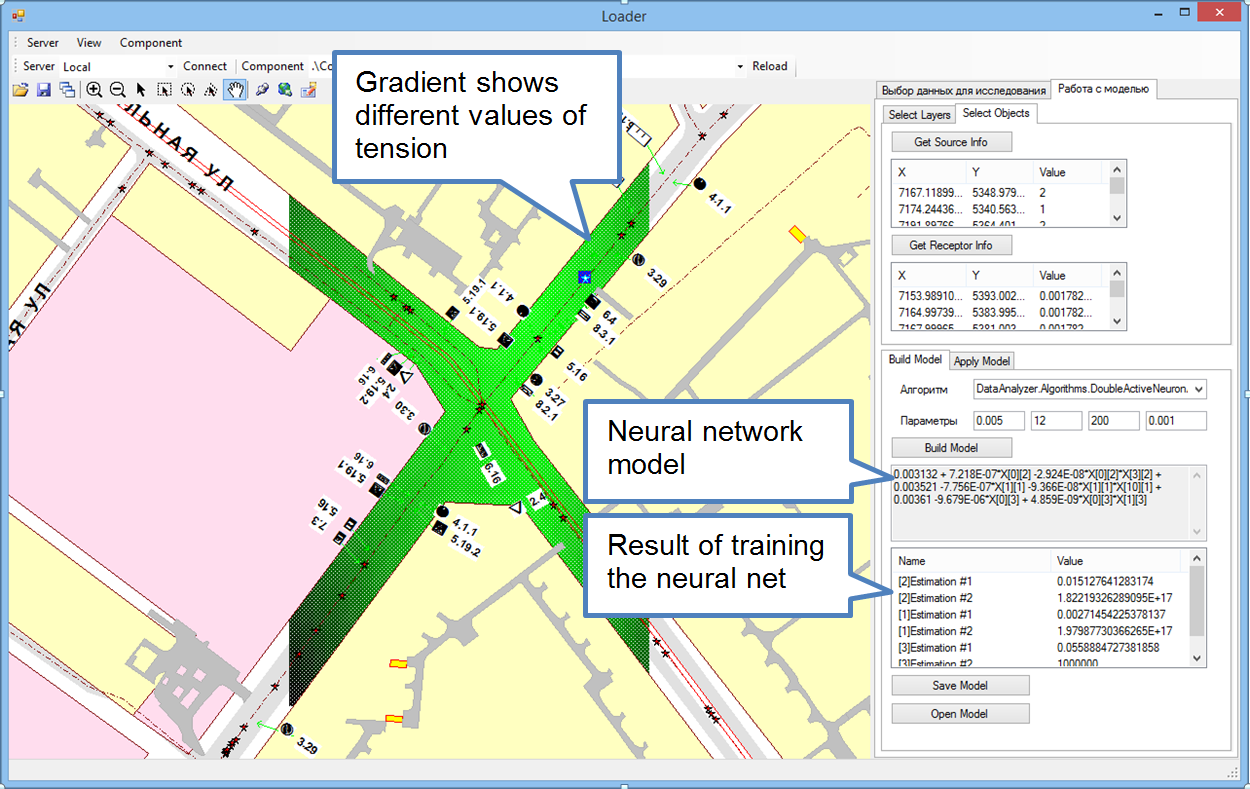
\includegraphics[width=0.99\textwidth, angle=0]{./scenarios/figures/samara_fig2.png}}%
{}
 %------------

% ##################################################################################################################